\documentclass[10pt]{article}
\usepackage{blindtext}
%\usepackage{geometry}
%\usepackage[englihs]{babel}
\usepackage{tikz}
\usepackage{varwidth}
\usepackage{capt-of}  
%\floatstyle{plain}
\usepackage{wrapfig}
\usepackage{caption}
\usepackage{subcaption}
%\usepackage[most,listings]{tcolorbox}%control boxds
%\usepackage{algorithm}
%\usepackage{algpseudocode}
%\usepackage{colcitepor}
%\usepackage{lipsum}%special stuff for text and math fonts
\usepackage{amsmath}
\usepackage{amssymb}
\usepackage{bbm}
\usepackage{wrapfig}
%\usepackage{tikz}
%\usetikzlibrary{arrows}
%\usepackage{lmodern}%fonts
%\usepackage[T1]{fontenc}
%\renewcommand*\familydefault{\sfdefault} % to get sans serif
%\usepackage{authblk}% author location
%\renewcommand*{\Affilfont}{\normalsize}
%\usepackage{breakcites}%bibliography and stuff
%\usepackage{booktabs}
%\usepackage{listings}
%\usepackage{epstopdf}
% alt: authoryear
%\usepackage[backend=biber, style=numeric, uniquename=false,doi=false,isbn=false, url=false]{biblatex}

\usepackage{hyperref}%hyperrects
\hypersetup{
colorlinks=true,
linkcolor=blue,
urlcolor=blue,
citecolor=blue,
}

\usepackage{parskip}
\setlength{\parskip}{\medskipamount}
\makeatletter 
\newcommand{\@minipagerestore}{
\setlength{\parindent}{15pt}
%\setlength{\parskip}{\medskipamount}
}
\usepackage[a4paper, margin=2cm,headsep=6pt]{geometry}
\usepackage{lineno}
\usepackage[english]{babel}
\usepackage{graphicx}
\usepackage{float}
\newcommand{\soptitle}{Computational analysis of ornament in Iznik ceramics}
\usepackage{fancyhdr}
\pagestyle{fancy}
\linespread{1.4}
\fancyhead[R]{CID YY5819}
\fancyhead[L]{Yuchen Yang}
\usepackage{csquotes}
\usepackage[backend=bibtex,style=authoryear]{biblatex}
\bibliography{Project_ProposalBib.bib}




\begin{document}
\begin{titlepage}
\begin{center}
\hrule
\vspace{2pt}
\hrule
\vspace{2cm}
\LARGE {\bf \underline{Project Proposal}}\\
\vspace{2cm}
\huge{\bf \soptitle}\\
\vspace{4cm}
\LARGE {\bf Yuchen Yang}\\
\large {\bf MRes Computational Method for Ecology and Evolution}\\
\vfill
\LARGE {\bf Supervisor: Prof. Armand Leroi}\\
\large {\bf Professor of Evolutionary Developmental Biology}\\
\large {\bf Department of Life Sciences}\\
\large {\bf Imperial College London}\\
\large {\bf a.leroi@imperial.ac.uk}
\end{center}
\hrule
\vspace{2pt}
\hrule
\end{titlepage}
\linenumbers

{\bf Keywords: }topic model, image segmentation, cultural evolution, Iznik ornament, taxonomy, visualisation

\section*{Introduction}

As Darwin noted in the \emph{The Descent of Man and Sexual Selection} (1871), animals and humans are often extravagantly ornamented. The human body is rather dull, but our extended phenotypes --- the artifacts we produce --- are not \parencite{Jones1856, Gombrich1994, Trilling2001}. Ornamental motifs --- e.g., the plumage of the the Argus pheasant and the tattoos of New Zealand Maori that Darwin discussed --- are, however, very complicated and hence hard to describe quantitatively (but see \cite{Tehrani2009} on Iranian carpets).

\begin{wrapfigure}{r}{10cm}
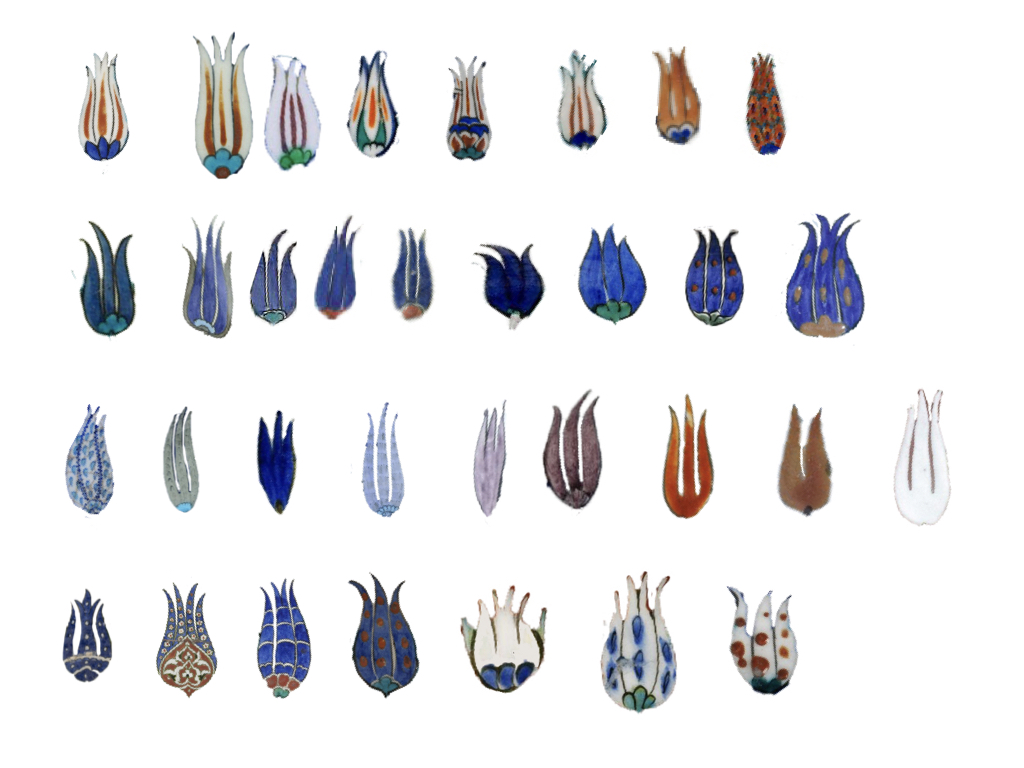
\includegraphics[width=10cm]{tulipcol}
\caption{A collection of tulips ---part of the vocabulary of Iznik ornament.}
\label{fig:tulipcol}
\end{wrapfigure}
This project applies various machine learning tools in order automatically identify and classify ornamental motifs, with the ultimate aim of studying their evolution.  It will focus on ceramics produced in the Turkish city of Iznik between roughly 1425 and 1625 \parencite{Atasoy1994}. These ceramics, which have very distinctive patterns, include the hundreds of thousands of tiles that still cover Ottoman public buildings in Istanbul. They are one of the triumphs of Islamic art.

The basis of the project is 465 images of Iznik ceramics culled from museum websites and monographs.  These ceramics display various stereotyped motifs:  tulips, carnations, ``saz'' leaves and so on (e.g., Figure \ref{fig:tulipcol}). The project has four aims: First, to develop an ornamental ``vocabulary'' --- a classification of motifs; second, to identify ornamental ``styles'' --- a classification of the various ways in which the words of the vocabulary are combined; third, to develop a method for automatically identifying motifs in ceramics; fourth to develop vizualizations of the results. 

%Current studies have provided a lot of opportunities to finish the above-mentioned tasks. In particular, Latent Dirichlet Allocation(LAD) could be used to understand the topic or the style of the ornament, and for a smooth and effortless process, a Mask-RCNN could help to find future homologous motifs from the ornaments.

%The project aims to develop a novel approach that could scale to analyse any ornamental arts using clustering, topic model, and image segmentation, resulting in a taxonomy of a set of a given input. the project would also provide an interactive visualisation where the taxonomy could be shown and played around with. the quantified data should be a great help to future studies of any cultural, developmental evolutionary subject.
\section*{Proposed Methods}
\paragraph{} The 465 images have already been manually segmented for three classes of motifs: carnations ($N=463$), tulips ($N=2067$) and saz leaves ($N=5030)$. Unsupervised machine learning (ML) methods will be used to classify these motifs into an ornamental ``vocabulary" --- sub-types based on their size, shape and colours. Topic analysis  will then be used to discover the styles of the artefacts (e.g., a tile or plate). These analyses are based on (laboriously) manually segmented motifs, but we would like to be able to extract them automatically, so I will develop supervised ML methods do so. Finally, I will develop visualization tools for the results. The project is ambitious, builds on much preliminary work; Table~\ref{Tab:methods} gives some details.

\begin{table}[ht]
\caption{Proposed methods}
\begin{tabular}{l|l}
\cline{1-2}
\small
\textbf{Discover the vocabulary} & Clustering (HCA, GMM, kmeans) based on the colour, shape, and size of motifs\\ \cline{1-2}
\textbf{Discover the grammar}  & Latent Dirichlet Allocation (LDA) topic analysis on artefacts \\ \cline{1-2}
\textbf{Image segmentation}   & Mask-RCNN development for automated motif recognition tasks\\ \cline{1-2}
\textbf{Visualisation}& Use D3, Processing and web languages to build a interactive platform for the results \\ \cline{1-2}
\end{tabular}
\label{Tab:methods}
\end{table}
\section*{Anticipated outcomes}

The anticipated outcomes of the project are as follows:

\begin{enumerate}
    \item An orthogonal classification of ornamental motifs into sub-classes based on colour, size and shape.
    \item An inital classification of artefacts into styles based on their motifs.
    \item A RCNN model capable of accurately segmenting tulips, carnations and saz leaves from Iznik ceramics.
    \item An interactive platform to showcase the results.
\end{enumerate}

The methods that I will develop here have several possible uses.  Most obviously, they can be used to document the evolution of Iznik ornament over the course of the 150 years or so that it flourished.  The sample of artefacts used here is too small to do this directly, however, the RCNN model will permit the automatic segmentation, and hence study, of the hundreds of thousands of tiles in Istanbul. Extending these method to other, related, decorative traditions will allow us to quantitatively study the origin and spread of ornamental motifs. Some of these originate in Ming China; others come from Persia or even ancient Egypt, and they continue to influence ornamental art to this day \parencite{Jones1856, Riegl1992, Brolio2016}. More generally, the methods that I will develop should be applicable to the study of ornament whereever it is found. For example, they may be useful for large-scale studies of the evolution of bird plumage. 


%Ornamental art is far more than just decorations, it is also a very important source to different studies: history, anthropology, developmental evolution, and so on \autocite{mitrache2012ornamental}, as it is a mirror for human activities and condensed the social and cultural elements\autocite{zerner1976alois}. Scholars have used connections between ornamental traditions to verify how different cultures are connected and communicated. For example, the influence of Ming porcelain Ottoman ceramics, especially during the Empire's height in the sixteenth century \autocite{carroll1999could}. The main challenge of studying the ornamental art, or any art at all, is to quantifying them, in a more systematic, automated way , and with the rapid development of the technology available, patterns on the ornament, colour usage, even the style can be extracted and analysed. 






\section*{Feasibility}
\paragraph{} 
\begin{figure}[H]
\begin{center}
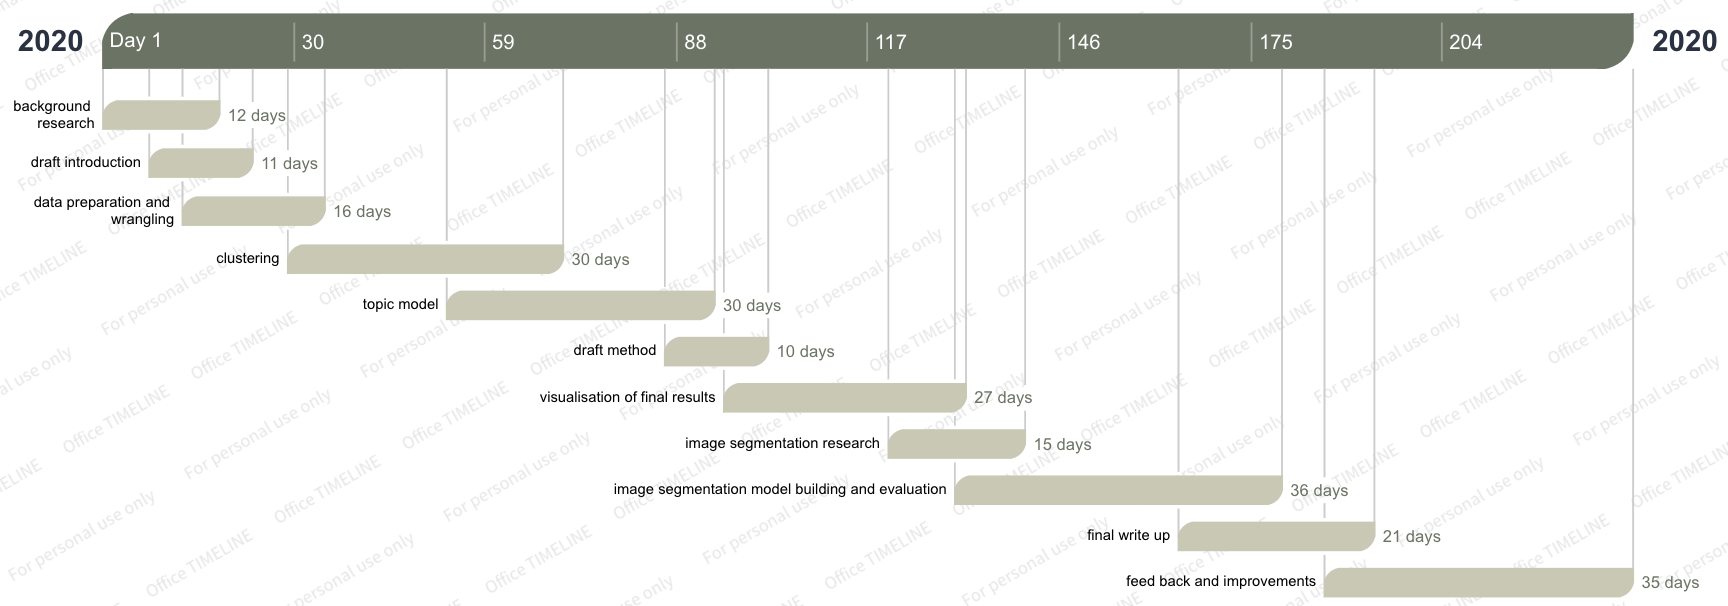
\includegraphics[scale=0.4]{Proposal/gantt.png}
\end{center}
\end{figure}
\section*{Budget}
Approximate budget listed below:\\
\pounds 150 - Monthly visit to South Kensington Campus, one return rail fare and two tube fares per visit\\
\pounds 200 - Potential computing power and hardware buying for image segmentation task\\
\pounds 150 - Potential visit to conferences and seminars 
\clearpage
\printbibliography
\end{document}